\documentclass[main]{subfiles}
\usepackage[]{workbook}
\numbering{ws1-7}

\begin{document}

\ifSubfilesClassLoaded{%
  \chaptermark{\chapterone}
}{}

\section{Upper Bounds and Error} \label{ws1-7}
\begin{framed}
\textbf{Lesson Goals:}
\begin{itemize}[parsep=0pt]
\item You should be able to understand and explain the error bound formulas for $L_n$ and $R_n$, including what they say, the notation they use, and the motivation behind the formulas.
\item You should be able to find upper bounds for functions and their derivatives on a given interval using various techniques, including the Triangle Inequality.
\end{itemize}
\end{framed}
\begin{enumerate}
\item Consider the function $f(x)=x^2\sin(x)$ on the interval $[0,10]$.

\begin{enumerate}
    \item \begin{problem}[\vfill]Using the skills you learned in Calc 1, how would you find the maximum value this function reaches on the interval?
    \end{problem}

    \begin{solution}
        To find the maximum value of the function on the interval, we would need to find all places where $f'(x)=0$ on the interval as well as the endpoints. $f'(x)=2x\sin(x)+x^2\cos(x)$. Setting this equal to 0, we would need to solve the equation $2x\sin(x)+x^2\cos(x)=0$, which is very difficult.
    \end{solution}
    \item \begin{problem}[\vfill]
        Part (a) turns out to be difficult. Could you instead find an \textit{upper bound} of this function on the interval? (An upper bound is a value larger than the function on the whole interval)
    \end{problem}

    \begin{solution}
        We know the largest value of $\sin(x)$ is 1, and the largest $x^2$ can be on $[0,10]$ is 100, so 100 is a reasonable upper bound. The actual maximum on this interval is 63.63, so this is indeed an upper bound.
    \end{solution}
\end{enumerate}
\pspace{\newpage}
\begin{framed}
    \textbf{\underline{Working with Absolute Values:}}\begin{itemize}
        \item $|AB|=|A||B|$
        \item $\left|\dfrac{A}{B}\right|=\dfrac{|A|}{|B|}$
        \item $|A+B|\leq |A|+|B|$   (Triangle Inequality)
        \item $|A-B|\leq |A|+|B|$   (Triangle Inequality)
    \end{itemize} 
\end{framed}
\item 
\begin{problem}
Find a practical upper bound for each of the following functions on the given interval.
\end{problem}

\note{Emphasize that we want them to be practical here.  Emphasize that finding maxima is brutal usually, but finding upper bounds is much easier. } 

\begin{enumerate}
	\item
  \begin{problem}[\vfill]
  $| 2\sin x + x^{2}| $   on the interval $[-3, 2]$
  \end{problem}
  
  \begin{solution}
  Many solutions are possible, but here is a nice one.\\
  By the triangle inequality, we always know that $$|2\sin x + x^2 | \leq |2\sin x| + |x^2| = 2|\sin x| + x^2$$
  For the values of $x$ in $[-3,2]$, the biggest that $x^2$ could possibly be is $(-3)^2$.  The biggest that $|\sin x|$ can be is 1.   So the function is certainly bounded as follows:
  $$|2\sin x + x^2 | \leq |2\sin x| + |x^2| = 2|\sin x| + x^2 \leq 2(1) + (-3)^2 = \boxed{11}$$
  Note that the function never actually gets this big.  There's a significant difference between \textbf{an upper bound} and \textbf{the maximum}! (Why do I call it ``the'' max, but ``an'' upper bound?)
  \end{solution}


  \note{I'm going to introduce the triangle inequality here without proof.}
  \item
  \begin{problem}[\vfill]
  $| \sin x  - x^{2}| $    on the interval $[0, 5]$
  \end{problem}

  \begin{solution}
  We again use the triangle inequality (beware that $|a-b|\leq |a| {\color{red}+} |b|$) and the fact that $x^2$ increases from $x=0$ to $x=5$ to bound as follows:
  $$| \sin x  - x^{2}| \leq |\sin x | + |x^2| \leq (1) + (5)^2 = \boxed{26}$$.
  \end{solution}

  \item
  \begin{problem}[\vfill]
  $|(x\sin x)(e^{-x} + x^{2})|$    on the interval $[1, 3]$
  \end{problem}

  \begin{solution} The absolute value of a product is the product of the absolute values, so we can bound each of the factors.  In the last factor, we use the triangle inequality, and note that $e^{-x}$ decreases from $x=1$ to $x=3$, so it's no bigger on the interval than $e^{-1} = 1/e  \leq 1$.
  $$ |(x\sin x)(e^{-x} + x^{2})| =  |x|\cdot|\sin x|\cdot|(e^{-x} + x^{2})|\leq (3) (1)(|e^{-1}| + |x^2|) \leq 3\cdot ( 1 + 9 ) = \boxed{30}$$
  \end{solution}


  \item
  \begin{problem}[\vfill]
  $\displaystyle \left| \dfrac{3\sin x - \cos x}{1+x} \right| $    on the interval $[1, 4]$
  \end{problem}

  \begin{solution}
  To find an upper bound for a fraction, find an upper bound for the numerator and a (positive) lower bound for the denominator. Notice that the denominator is no smaller than $1+(1) = 2$ on the interval.  So, using the triangle inequality in the numerator,  we can bound as follows:

  $$\left| \frac{3\sin x - \cos x}{1+x} \right|  \leq \frac{3|\sin x| + |\cos x|}{2} \leq \frac{3+1}{2} = \boxed{2}$$

  \end{solution}
  \end{enumerate}
  \pspace{\newpage}
   \item 
  \begin{problem}[\vfill]
  Suppose we use a left-hand Riemann sum with $n$ slices ($L_{n}$)
  to approximate $\displaystyle{\int_{a}^{b} (1+3x)\ dx}$.  Find a formula for the error in
  your approximation.  (You should begin with a picture. Your answer should be in terms of $a$, $b$, and $n$.)
  \end{problem}

  \note{ GOOD QUESTIONS TO ASK after they've worked on this:\\ What is it about this scenario that makes it possible to get a
  formula for the exact error?  Also explore the various features of the 
  formula -- where does the $3$ come from? why is it reasonable that
  there's an (a-b) in the numerator and and $n$ in the denominator?
  How does this verify our intuition that the approximation gets better 
  as we take larger and larger $n$?}



  \begin{solution}
  In the sketch, we see something like what the scenario would look like with $5$ slices.  

  
\includegraphics[width=2in]{ws/images/linear-error}

  The error is the total area of the triangles.  Each of these would have width $\Delta x = \frac{b-a}{n}$, and each of them has height $\Delta y$: notice that $\frac{\Delta y}{\Delta x} = 3$, since the slope of the line is $3$, so $\Delta y = 3\Delta x$.  So the total area of the $n$ triangles is:
  $$n \cdot (\text{area of one triangle}) = n 
  \cdot \frac12 bh = n 
  \cdot \left(\frac12 \Delta x \Delta y\right) = n \cdot \frac{1}{2}\left(\frac{b-a}{n}\right)\left(3\cdot \frac{b-a}{n}\right) = \boxed{\frac{3(b-a)^{2}}{2n}}$$
  Notice that this is the exact error, and we were able to compute it because the function is so simple.  The $3$ in the numerator above is the slope of the line.  Would a steeper line have a bigger or smaller error? What happens to the error if we use more slices? What happens to the error if we use the same number of slices, but we're looking at a much larger interval $[a,b]$?

  \end{solution}



%Problem 2
  \item
  \begin{problem}
    What happens if instead we are trying to approximate $\displaystyle I = \int_a^b (mx+c) \ dx$ using $L_n$, i.e., generalizing the problem above by looking at the linear function $g(x) = mx + c$.  
  \end{problem}

  \begin{enumerate}
    \item 
    \begin{problem}[\vfill]
    Find a formula for $|L_n - I|$, the error in the $L_n$ approximation, that generalizes the formula you found in question \#1.
    \end{problem}

    \begin{solution}
    The only change is that the height of each triangle is now $\Delta y = m\Delta x$, as the slope of the line has changed.  The total error is thus
    $$\boxed{\frac{m(b-a)^{2}}{2n}}.$$
    \end{solution}

    \item 
    \begin{problem}[.7in]
    What does it mean to be looking at $|L_{n} - I |$ rather than simply at $L_{n}-I$?
    \end{problem}

    \begin{solution}
    By looking at the absolute value, we are considering only the size of the error.  The quantity $|A-B|$ is the distance between $A$ and $B$.   (Try this with a few different numbers, say $A=2$ and $B=7$  or $A=-5$ and $B=2$ to see what I mean.)  So $|L_{10} - I|$ is ``how far the approximation is from the actual value''.  Notice that in this slightly more general case, $L_n$ can be an overestimate for $I$ (if $m$ is negative) or an underestimate (if $m$ is positive).  So $L_n-I$ could be positive or negative, but the size of the error is what's most useful.
    \end{solution} 


  \end{enumerate}
  \pspace{\newpage}
\item \begin{problem}[\vfill]
    Use a similar strategy to get an upper bound on the error of approximating $I=\displaystyle\int_1^4\sqrt{x}\,dx$ using $L_3$. 
\end{problem}

\begin{solution}

Below, we see the area under the square root function approximated by $L_3$. We can see that the error is white region between the rectangles and the curve.
\begin{center}
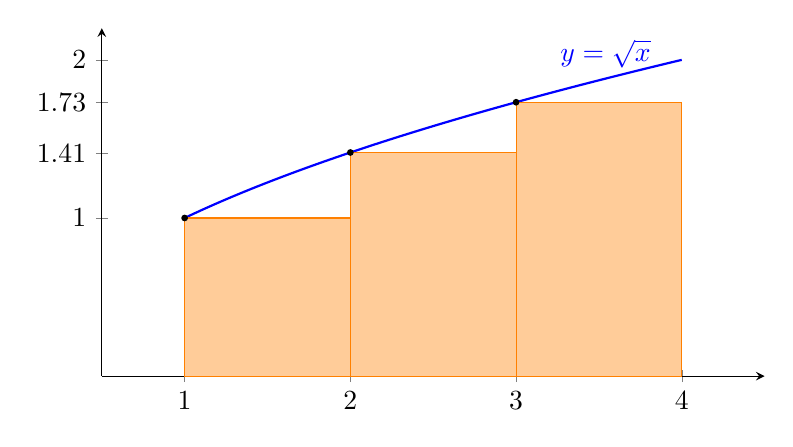
\begin{tikzpicture}
  \begin{axis}[
      axis lines=middle,
      xmin=0.5, xmax=4.5,
      ymin=0, ymax=2.2,
      xtick={1,2,3,4},
      ytick={1,1.41,1.73,2},
      width=10cm, height=6cm,
      domain=1:4,
      samples=100
    ]

    % Plot sqrt(x)
    \addplot [blue, thick] {sqrt(x)} node[pos=0.85, above] {$y = \sqrt{x}$};

    % Rectangle 1: [1,2], height = sqrt(1) = 1
    \addplot [
      ybar interval,
      bar width=1,
      fill=orange, fill opacity=0.4, draw=orange
    ] coordinates {(1,1) (2,1)};

    % Rectangle 2: [2,3], height = sqrt(2)
    \addplot [
      ybar interval,
      bar width=1,
      fill=orange, fill opacity=0.4, draw=orange
    ] coordinates {(2,{sqrt(2)}) (3,{sqrt(2)})};

    % Rectangle 3: [3,4], height = sqrt(3)
    \addplot [
      ybar interval,
      bar width=1,
      fill=orange, fill opacity=0.4, draw=orange
    ] coordinates {(3,{sqrt(3)}) (4,{sqrt(3)})};

    % Optionally, put points at key values
    \addplot[only marks, mark=*, mark size=1pt] coordinates {(1,1) (2,{sqrt(2)}) (3,{sqrt(3)})};
  \end{axis}
\end{tikzpicture}  
\end{center}

It would be difficult to find the exact error by finding the area of these curved regions. Instead, we can get an upper bound of the error by forming a larger triangle, like we did in the last parts. Using the steepest slope on the interval, we can make a triangle larger than the actual error, as the image below shows.

\begin{center}
     
\includegraphics[width=2in]{ws/images/square root error.png} 
\end{center}

The steepest part of the slope is the left most point. $f'(x)=\frac{1}{2\sqrt{x}}$. For the first triangle the area is then $\frac{1}{2}(1)\frac{1}{2}=\frac{1}{4}$. Thus, an upper bound of the error is $\frac{1}{4}+\frac{1}{4\sqrt{2}}+\frac{1}{4\sqrt{3}}$. For an easier upper bound, albeit less accurate, you could use the largest slope on the whole interval for each triangle. This is quicker to compute, and is how we compute the error bound formula below.
\end{solution}
\end{enumerate}

\begin{framed}
\textbf{\centerline{Error Bounds in Numerical Approximations}}
Let $ \displaystyle{I = \int_a^b  f(t)\,dt}$ and assume $f$ has a continuous derivative. Then the errors in using left and right hand sums can be bounded as follows:

\begin{multicols}{2}

\begin{center}
$|L_n - I | \leq \displaystyle \frac{  M_{(1)} (b-a)^2}{2n}$      
  
  
$|R_n - I|  \leq \displaystyle \frac{  M_{(1)} (b-a)^2}{2n}$
\end{center}


\end{multicols}
where $M_{(1)}$ is an upper bound for  $|f'|$ on $[a,b]$.

\end{framed}
 \end{document}